\chapter{Optimization of Mobile Communication Systems}\label{ch:monster}

Mobile Communication systems (or Cellular Networks) have become an essential part of modern society. For the better parts of 2 decades, the systems we use in our daily lives have evolved continuously, mostly behind the scenes, but also directly observable for everyone. The introduction of smartphones have required a revolution to existing mobile communication systems and have brought us technologies such as \gls{lte} $4$G and the to-be-deployed in the nearest future \acrfull{nr}. The content of these systems is probably one of the greatest engineering feats achieved in modern times. Such systems are increasingly complex, and future systems will most definitely introduce more complexity in order to increase capacity for the end-users efficiently. Behind this complexity resides the wireless transmission over the air that is the backbone of the systems. By understanding the fundamental physical properties of wireless transmission, the systems and sub-systems of existing technologies have been designed to very effectively transmit and receive signals over long distances. Understanding the wireless channel satisfactory has been a long-standing engineering achievement and has been improved immensely for these modern systems compared to just a few decades ago. The key to further improvement of these systems is by understanding every little detail that makes up the complex and mysterious act that is wireless transmission. So far, the working and operational systems that are deployed and used throughout the world is a manifest to the fundamental understanding of wireless transmission. 

As with any communication system, it is relevant to recall the well-known Shannon–Hartley theorem \cite{Tse2005FundamentalsCommunication}.

\begin{equation}\label{eq:shannon}
    C = B \log_2 \left( 1 + \frac{S}{N} \right)
\end{equation}

The theorem describes the information rate, also known as capacity $C$, is determined by 1) The so-called bandwidth $B$, 2) the received signal power $S$ and 3) the noise of the communication channel $N$. The Shannon-Hartley theorem determines the fundamental limits of capacity and has so far not been proven wrong. If the conditions of the communication channel are static and constant, the only way to increase capacity is by 1) increasing bandwidth and 2) increasing the signal received power.

Increasing bandwidth can be done by introducing new carrier frequencies, as is the case with \gls{lte} and \gls{nr}. A multitude of frequencies is deployed in the current cellular systems to increase the necessary capacity required for users \cite{Goldsmith2005WirelessCommunications, Molisch2007}. For this, we look towards the current and future of cellular networks in terms of so-called \gls{h-udn}.


% \begin{itemize}
%     \item Introduce the concept of cellular networks in broad strokes 
%     \item Mention capacity is dependent on two things, bandwidth, receiver signal power and the noise level
%     \item Introduce provisioning of systems and the relation to capacity
%       \item introduce the concepts of heterogeneous cellular networks
%     \item More capacity is always desired but comes at an expensive cost of deployment
%     \item optimisation of deployment is paramount to ensure reliable capacity and connectivity 
% \end{itemize}

\section{Heterogeneous Cellular Networks}
\gls{h-udn} also termed just Heterogeneous Cellular Networks, is a modification for improving the capacity of existing systems. Classical cellular networks consist primarily of centralised base stations effectively providing both coverage and capacity solutions to all users localised in the site. By doing so, the bandwidth and thus capacity is essentially limited by the base station. Both \gls{lte} and \gls{nr} seek to densify the cellular network architecture to improve bandwidth, and the channel conditions effectively increasing the available capacity. The densification in \gls{h-udn} consists specifically of introducing additional relays, and base station with reduced antenna arrays into the existing site. These are termed micro, pico and femtocells, depending on the deployment and overall requirements \cite{Yunas2015, Ge2016}. The result of this is effectively a reduction in the inter-site distance between the terminals and the deployed base stations. Such a case is depicted in Fig. \ref{fig:hudn_drawing}. The modification is furthermore to accommodate a large amount of available bandwidth in \gls{mmwave} frequencies. The use of \gls{mmwave} is expected to be an essential part of \gls{nr} solutions enabling massive capacity boosts. However, \gls{mmwave} suffer over longer distances to increased path loss and reduced penetration properties. By reducing the inter-site distance in future \gls{h-udn}, novel solutions such as \gls{mmwave} is feasible. 

\begin{figure*}
    \centering
    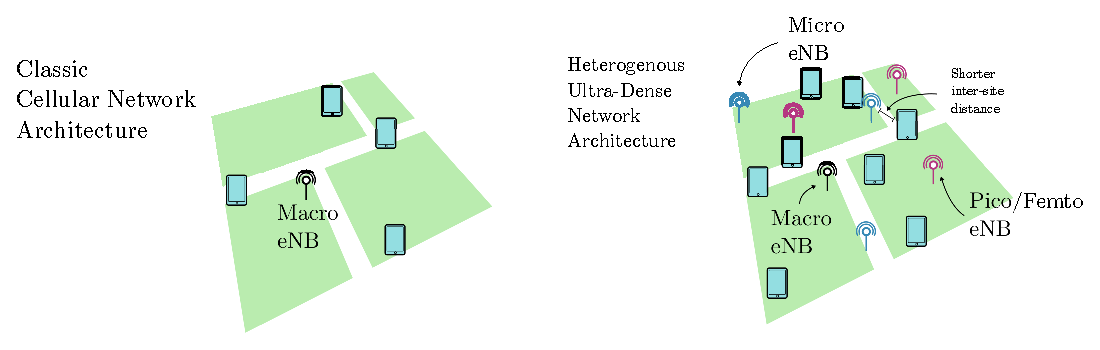
\includegraphics{chapters/part_pathloss/figures/hudn_drawing.eps}
    \caption{Additional sites with different transmissions frequencies are added to the existing network architecture to boost capacity.}
    \label{fig:hudn_drawing}
\end{figure*}


A classic cellular architecture usually consists of a single Macro base station that is tasked with supplying both coverage and capacity. In \gls{h-udn} such centralised base stations are expected only to handle control signals and wide-area low capacity coverage. The smaller base stations are thus tasked with the majority of user data management and the overall capacity. The necessary evolution and deployment of such systems are inevitably subject to complex deployment and management situations. The authors outline this in \cite{Taufique2017} that discuss the challenges and opportunities associated with the planning of such complex systems. The authors discuss the severe need for accurate models for the many aspects of such systems, including energy management, interference modelling, and wireless channel models amongst many others. 




\section{Optimization of Mobile systems}


Two phases describe the life-cycle of mobile communication systems. Before deployment (the planning phase) or during operation (optimization phase) \cite{Taufique2017}. In literature, it is found that the term \emph{optimization phase} is used to describe when the network has been deployed and is operational. However, in this dissertation, the term \emph{optimization} is used to define the improvement of a specific situation or resource. For instance, the planning phase can be optimised to ensure that the future addition of small cells and other unplanned deployments can be achieved without fundamental challenges related to the deployed network. Classic planning techniques are primarily focused on the optimisation of the number of base stations and their location. This has later evolved into a multitude of parameters to be considered. For instance, transmission specific parameters such as antenna tilt, transmission power and others can be used in the planning process to optimise the coverage and capacity of the system. With the emerging technologies of $4$G and $5$G, the planning phase have been extended with an extensive list of parameters  \cite{Taufique2017}. For instance, new capacity improving solutions such as \gls{mimo} require constant configuration and optimisation to ensure the maximum efficiency of the systems is utilised. The evolving complexity of these systems require \glspl{mno} to approach cellular planning differently. This have pushed so-called \gls{son} features to be an essential part of deployment and operation of future mobile communication systems. Additionally, and considered beyond the scope of this dissertation, is network virtualisation and \gls{sdn} methodologies  \cite{Taufique2017}.


In short and brief terms, \gls{son} is the automatization and self-configuration of processes related to the planning and operation of mobile networks. The features of \gls{son} is to ensure that mobile networks are cost-efficient as additional solutions for improving capacity make their way into existing systems. This can be achieved at many levels, for instance, by having a standardised and almost autonomous procedure for cellular deployment that optimise all associated parameters. An overview of \gls{son} features can be found in \cite{Jorguseski2014Self-organizingTrends} and references herein.

\acrlong{son} require intelligent methodologies for effectively providing with the much-needed intelligence. Learning methodologies, as provided by \acrfull{ml} is encompassed to fulfil these requirements. A comprehensive study of \gls{ml} applied for \gls{son} can be found in \cite{Klaine2017ANetworks}. 

In any case, \gls{son} features or not, the optimisation of mobile communication systems is effectively also a result of obtaining the necessary data representative of the deployment, or in the case of the planning phase to-be deployment. This can either be done through measurements, which is limited to deployed networks, or simulations. Simulations have over the recent years sparked an increasing amount of research papers and is a core technique for the optimisation of cellular networks and research hereof. Regardless, radio measurements is a key and necessary element for the performance evaluation of cellular networks and even more so with increased network complexity. Obtaining such measurements can be done with regular and frequent \emph{drive tests}. However, as the complexity of these systems increases the drive testing in itself becomes increasingly expensive. 

\subsection{Drive testing}\label{sec:drive_testing}

\begin{figure}
    \centering
    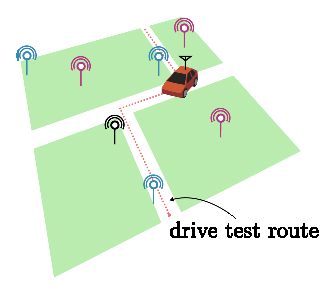
\includegraphics[width=.5\textwidth]{chapters/figures/drive_test_illustration.eps}
    \caption{Drive testing is an effective way of obtaining radio measurements, but time exhaustive}
    \label{fig:my_label}
\end{figure}


Drive testing consists simply of attaching an antenna on top of a vehicle and driving around areas of deployment. Examples of such data sets can be found in Appendix \ref{app:drive_test_study_2017} and \ref{app_drive_test_study_2020}. Obtaining drive test measurements is a costly affair as deployment regions can cover large or hard-to-reach areas. Optimising the drive test procedure have been attempted by utilising hardware in the loop and 3D acceleration \cite{Charitos2017} with promising results. However, the default solution is to practically fit a car with the right equipment and drive around. Drivable roads effectively limit the granularity. Measurement solutions exist for doing it on foot and are useful in non-drivable areas and indoor coverage situations \cite{ROMESmanual}. 

\subsection{\glspl{kpi}}
Depending on the mobile communication system, the \gls{kpi} differ. For \gls{lte} and \gls{nr} an extensive list of relevant metrics exist. For this dissertation the focus in on the following reference signal based metrics
\begin{itemize}
    \item \gls{rsrp}
    \item \gls{rssi}
    \item \gls{rsrq}
\end{itemize}

A set of so-called reference signals are used to infer the value of the above metrics. Additionally to these, \gls{sinr} is a commonly used metric and is a direct indication of the achievable information rate for a given transmission link. The freqeuncy resuse of modern mobile communications introduce interference between neighbouring sites. The metric of \gls{rsrp} is the measure of reference signal power for a single base station. The reference signals between neighbouring base stations differ and therefore an independent measurement of the received power can be obtained. This is different for \gls{rssi} which contains the average power of all reference signals observed. Therefor, \gls{rssi} is the measure of neighbouring base stations within reach of the receiver. \gls{rsrq} is fraction between the \gls{rsrp} and \gls{rssi} and is thus a metric of infering the interference caused by neighbouring base stations. A detailed description of these metrics can be found in \cite{Molisch2007}.

By inspecting the resulting drive tests, improvements to existing deployments can be made. For instance, if any coverage holes or interference sources are identified, they can be remedied to improve capacity and coverage and thus the resulting customer experience. Drive tests are a common practise utilised by \gls{mno} to evaluate the efficiency of deployments continually. Performing drive testing is an extremely costly affair, and there is a significant opportunity to cut both capital and operational costs by reducing the number of needed drive tests. Solutions related to reducing drive testing is termed \gls{mdt}


\subsection{Minimization of drive testing}
\gls{mdt} is introduced with Release 10 of \gls{lte} and introduces principles for minimising the required drive testing. The approach uses reports from the attached \glspl{ue} to evaluate not only the coverage but also the capacity of mobile communication systems. In essence, the concept consists of having the \gls{ue} transmit back a report detailing necessary and important \glspl{kpi} such as \gls{rsrq} and \gls{rsrp} among others. By combining these measured parameters with a localisation metric, so-called \emph{radiomaps} can be constructed. 

In the case of radiomaps, this can be used in combination with so-called \emph{kriging} methodologies enabling interpolation between the received \gls{kpi} reports. By doing so, useful approximations of capacity and coverage can be estimated given only a few measurements (sparse). By doing so, it enables the deduction and analysis of any existing coverage holes and other coverage impairments \cite{Bi2018EngineeringManagement}. 

However, such methods are dependent on accurate positioning. \gls{mdt} as per Release 10 \cite{3GPP2017} can utilize \gls{gnss} solutions if present in the \gls{ue}. However, doing so have to significant drawbacks \cite{Schloemann2016}. 

1) The accuracy of \gls{gnss} when not under open sky suffers from substantial inaccuracies. These inaccuracies are notably the case for indoor scenarios. 

2) The power draws from any \gls{gnss} solutions drain the battery of \glspl{ue} which is not ideal. 

Additionally, \glspl{ue} produce a noticeably difference in the \glspl{kpi} due to different quality electronics and antenna sub-systems \cite{Karstensen2017}. This further complicates the procedure of estimating coverage maps.

The localisation of users is paramount to minimising drive testing. Localisation is not only a necessary parameter for \gls{mdt} but also a necessity for emergency services to localise users in distress. One solution for doing so is utilising the so-called \gls{otdoa}. The parameter is useful for localising users in the radio environment \cite{Johansson2012} and can be used effectively for \gls{mdt} reports. However, utilising such a parameter can yield \emph{overly-optimistic expectations} when introducing a distinct increase in the number of neighbouring base stations \cite{Sivers2015, Schloemann2016}. 

While \gls{mdt} is an efficient way of obtaining measurements for current and future cellular systems, a traditional way of evaluating coverage and capacity include the use of so-called \emph{simulation environments}. 

\subsection{Simulation}
Mobile networks are costly to deploy; thus, network simulation is a powerful and necessary tool for the optimisation and development of future cellular networks. Simulators enable insights that may otherwise be infeasible to obtain through practical deployments. For instance, this includes the estimation of coverage and capacity for a given propagation scenario. It provides with essential insights into, for instance, the optimum locations of the required base stations. Or the upper and lower capacity bounds. By doing so, the properties of the systems can be evaluated and reevaluated to accommodate any needs related to, for instance, existing customers or economic considerations. Network simulators are essential for the future of wireless systems as also indicated by the authors in \cite{Cavalcanti2017}. 

Additionally, as this dissertation is focused around the application of \gls{dl} model, it is logical to use simulation tools for not only data generation but also studying existing optimisation procedures. During the development of the presented models and solutions throughout this dissertation, a significant number of various implementations were completed. It quickly realised that such implementations might be useful for the community. Consequently it was made open-source \cite{monster}$^1$.
\begin{marginfigure}
1 The tool found in \cite{monster} implements the majority of the empirical path loss models found in Chapter \ref{ch:channelmodellingbasics}. A majority of figures throughout this dissertation is created with the use of the framework. The framework is engineered to be modular and has significant ease of implementation for additional modules and extensions. A guide for contribution can be found in the repository. The foundation of the framework is built on the \texttt{LTE toolbox} by MathWorks. This includes also the specific implementations of the fast-fading models of \gls{tdl} and \gls{cdl} as briefly introduced in Chapter \ref{ch:channelmodellingbasics}.
\end{marginfigure}


\subsection{Channel models}

Radio propagation models or wireless channel models is an essential part of the design of mobile communications systems, and future systems even more so. The multitude of frequencies, bandwidths, and overall transmission complexity is subject to many different and complex interactions in the radio environment. Knowing how specific configurations of the communication system perform is essential to optimisation in both the planning and deployment phase of mobile networks. Models for emulating and simulating wireless channels have been an essential part of designing cellular systems as configurations, and new technologies can be tested cost-effectively. Statistics of wireless impairments can be deduced from obtained measurements (for instance, by using drive testing) and can be used in the planning and development of mobile communication solutions. The use of such statistics is a standard procedure and has resulted in the highly effective and straightforward \emph{empirical} wireless channel models. 

Channel models have been an essential element in the planning of mobile communication systems for a very long time \cite{Taufique2017, Cavalcanti2017}. By estimating and approximating the impact of the wireless channel changes and optimisation of the communication system can be achieved. For instance, channel models may enable the study of coverage for a given set of deployed cells. If the accuracy of the channel models are high, and coverage holes in the deployment can be identified, the deployment may be optimised to improve capacity and coverage. All this without doing expensive drive testing.

Modelling wireless interactions is a complex task, and for this reason, a multitude of channel models exist, with different model complexity. The study of the wireless channel has resulted in a few \emph{default} channel models—each with a different purpose. A brief introduction to such models can be found in Chapter \ref{ch:channelmodellingbasics}.

The introduction of \gls{h-udn} and \gls{mmwave} impose new stringent requirements for channel models and the applications for use in \gls{nr} mobile networks 
\cite{Wang2018}. Not only is a wide range of supported frequencies required, but also, more importantly, a wide range of propagation scenarios are needed to improve the performance of the models. 

The applications of channel models are expected not to be limited to the planning and deployment phases of future mobile communication systems. Recently, the talks of so-called anticipatory- and cognitive-networking is expected to be a primary driver for future technologies such as advanced \gls{son} techniques (for improving the optimisation capabilities of cellular systems) and autonomous vehicles \cite{Bui2017ATechniques, Zhang2018}. So, it can be found that accurate wireless channel models are essential to the optimisation of current systems but also a necessity for future systems. The trend of new and improved wireless channel models are furthermore essential to enable the development of solutions for future mobile communication systems. This results in the development of novel methods and solution to not necessarily require a full measurement campaign, which is time-consuming and expensive. Improved channel models thus effectively lead to improved solutions for future mobile communication systems. However, it is essential that improvements to current channel models also consider computational complexity, not only concerning the required data but also in terms of the resulting computational run-times.


\section{Is Deep Learning applicable to Mobile Communication systems?}
\gls{ml} has been hailed to be a key enabler in future mobile communication systems due to the capabilities of learning complex mapping functions. \gls{ml} is capable of learning complex functions through data observations that may otherwise be challenging to engineer. As discussed through the majority of this chapter, future mobile communication systems consist of many complex interactions and sub-systems. Therefore \gls{ml}-based solutions are regarded as an essential element in future cellular systems \cite{Li2017IntelligentIntelligence, Klaine2017ANetworks}. 
 
The specific capabilities of \gls{ml}-based solutions have been shown in recent literature. For instance, in \cite{OShea2017, Dorner2018, Aoudia2018} the authors show how a \gls{dl} model (a subfield of \gls{ml}) can be trained to learn the entire physical layer of a wireless communication system, in what they term \emph{end-to-end} learning. The adaptive model is capable of learning a full transmitter and receiver implementation yielded by the conditions of a channel model using a \gls{nn}. In other words, all sub-systems in a regular \gls{ofdm}-based receiver and transmitter can be learned by obtaining the right measurements. While this may not be feasible for practical systems, it shows the use case of \gls{dl} models in wireless communication system design.


A massive survey paper discussing the use cases of \gls{ml} in wireless network systems can be found in \cite{Zappone2019}. The authors discuss \emph{\gls{ai}-based Wireless Networks} that is driven entirely on data. The authors discuss the future of wireless networks and argue that these networks will consist of extreme complexity which means traditional approaches to network design and management are ineffective or as they print it: \emph{no longer adequate}. This particular point is the point that this chapter is trying to underline and define from the perspective of mobile communication systems. 


This dissertation will attempt to answer the question \emph{"Is Deep Learning applicable to Mobile Communication systems?"} through several novel \gls{dl} applications for mobile communication systems. The state of current mobile communication systems is massive and complex. Therefore, the provided answers will only be related to a reduced scope of applications. The physical layer is identified as a promising area for \gls{dl} applications, due to 1) the data quantities provided by radio measurements, and 2) the unknown characteristics (to some extend) of the radio propagation environment.  In chapter \ref{ch:mlbasics} a very brief introduction to the overwhelming world of \gls{ml} and \gls{dl} is given along with useful literature. 